\documentclass{article}
\usepackage{cmap}
\usepackage[utf8]{inputenc}
\usepackage[english,ukrainian]{babel}
\usepackage{graphicx}
\usepackage{geometry}
\usepackage{listings}
\usepackage{amsmath}
\usepackage{float}
\geometry{
	a4paper,
	left=20mm,
	right=20mm,
	top=20mm,
	bottom=20mm
}
\lstset{
	language=c,
	tabsize=4,
	keepspaces,
	showstringspaces=false,
}
\graphicspath{ {./pictures} }
\setlength{\parindent}{4em}

\newcommand\subject{Операційні системи}
\newcommand\lecturer{старший викладач кафедри ПЗ\\Грицай О.Д.}
\newcommand\teacher{старший викладач кафедри ПЗ\\Грицай О.Д.}
\newcommand\mygroup{ПЗ-22}
\newcommand\lab{5}
\newcommand\theme{Багатопоточність в операційній сисемі WINDOWS. Створення,
	керування та синхронізація потоків}
\newcommand\purpose{Ознайомитися з багатопоточністю в ОС Windows. Навчитись
	реалізовувати розпаралелення алгоритмів за допомогою багатопоточності в ОС
	Windows з використанням функцій WinAPI. Навчитись використовувати різні
	механізми синхронізації потоків}

\begin{document}
\begin{normalsize}
	\begin{titlepage}
		\thispagestyle{empty}
		\begin{center}
			\textbf{МІНІСТЕРСТВО ОСВІТИ І НАУКИ УКРАЇНИ\\
				НАЦІОНАЛЬНИЙ УНІВЕРСИТЕТ "ЛЬВІВСЬКА ПОЛІТЕХНІКА"}
		\end{center}
		\begin{flushright}
			Інститут \textbf{КНІТ}\\
			Кафедра \textbf{ПЗ}
		\end{flushright}
		\vspace{200pt}
		\begin{center}
			\textbf{ЗВІТ}\\
			\vspace{10pt}
			До лабораторної роботи № \lab\\
			\textbf{На тему}: “\textit{\theme}”\\
			\textbf{З дисципліни}: “\subject”
		\end{center}
		\vspace{112pt}
		\begin{flushright}
			
			\textbf{Лектор}:\\
			\lecturer\\
			\vspace{28pt}
			\textbf{Виконав}:\\
			
			студент групи \mygroup\\
			Коваленко Д.М.\\
			\vspace{28pt}
			\textbf{Прийняла}:\\
			
			\teacher\\
			
			\vspace{28pt}
			«\rule{1cm}{0.15mm}» \rule{1.5cm}{0.15mm} 2022 р.\\
			$\sum$ = \rule{1cm}{0.15mm}……………\\
			
		\end{flushright}
		\vspace{\fill}
		\begin{center}
			\textbf{Львів — 2022}
		\end{center}
	\end{titlepage}
		
	\begin{description}
		\item[Тема.] \theme.
		\item[Мета.] \purpose.
	\end{description}

	\section*{Лабораторне завдання}
	\begin{enumerate}
		\item Реалізувати заданий алгоритм в окремому потоці
		\item Виконати розпаралелення заданого алгоритму на 2, 4, 8, 16 потоків
		\item Реалізувати можливість зупинку роботи і відновлення, зміни пріоритету
		певного потоку
		\item Реалізувати можливість завершення потоку
		\item Застосувати різні механізми синхронізації потоків. (Згідно запропонованих
		варіантів)
		\item Зобразити залежність час виконання – кількість потоків (для випадку без
		синхронізації і зі синхронізацією кожного виду).
		\item Результати виконання роботи відобразити у звіті
	\end{enumerate}
	\begin{center}
		Семафор, Інтерлок-функції
	\end{center}

	\section*{Хід роботи}	
	\begin{lstlisting}
#include "mainwindow.h"
#include "./ui_mainwindow.h"
#include <windows.h>
#include <stdio.h>
#include <iostream>
#include "QDebug"
#include "QLineEdit"
#include "QTimer"

struct PARAMETERS {
	int i;
};

struct threadStatus {
	DWORD threadID;
	int task;
};

HANDLE ghSemaphore;
DWORD WINAPI ThreadProc(LPVOID);

int* array;
int N;
int maxSemCount;
int threadCount = 0;
LONG sum = 0;
HANDLE* aThread;
DWORD ThreadID;
threadStatus* s;

MainWindow::MainWindow(QWidget *parent)
: QMainWindow(parent)
, ui(new Ui::MainWindow)
{
	ui->setupUi(this);
	QTimer *timer = new QTimer(this);
	connect(timer, &QTimer::timeout, this, &MainWindow::abc);
	timer->start(100);
}

MainWindow::~MainWindow() {
	for (int i = 0; i < threadCount; i++)
	CloseHandle(aThread[i]);
	
	CloseHandle(ghSemaphore);
	delete ui;
}

void MainWindow::on_pushButton_clicked() {
	ui->pushButton->setDisabled(true);
	N = ui->le_length->text().toInt();
	threadCount = ui->le_threads->text().toInt();
	s = new threadStatus[threadCount];
	maxSemCount = ui->lineEdit->text().toInt();
	aThread = new HANDLE[threadCount];
	array = new int[N];
	
	ghSemaphore = CreateSemaphore(
	NULL,
	maxSemCount,
	maxSemCount,
	NULL);
	
	if (ghSemaphore == NULL) {
		qDebug() << "CreateSemaphore error: " << GetLastError();
		return;
	}
	QStringList l;
	l << "IDLE" << "LOWEST" << "BELOW_NORMAL" << "NORMAL" << "ABOVE_NORMAL" << "HIGHEST";
	ui->prio2->addItems(l);
	QStringList list;
	for (int i = 0; i < threadCount; i++) {
		list << QString::number(i);
		
		PARAMETERS* p = new PARAMETERS{ i };
		s[i] = threadStatus { 0,0 };
		aThread[i] = CreateThread(
		NULL,
		0,
		(LPTHREAD_START_ROUTINE)ThreadProc,
		p,
		NULL,
		&ThreadID);
		if( aThread[i] == NULL ) {
			qDebug() << "CreateThread error: " << GetLastError();
			return;
		}
	}
	ui->sus->addItems(list);
	ui->res->addItems(list);
	ui->kill->addItems(list);
	ui->prio1->addItems(list);
}

void MainWindow::abc() {
	ui->le_sum->setText(QString::number(sum));
	ui->tableWidget->setColumnCount(3);
	ui->tableWidget->setRowCount(0);
	
	for (int i = 0; i < threadCount; i++) {
		ui->tableWidget->insertRow(i);
		for (int j = 0; j < 3; j++) {
			QTableWidgetItem * item = new QTableWidgetItem();
			item->setTextAlignment(Qt::AlignCenter);
			switch (j) {
				case 0:
				item->setText(QString::number(s[i].threadID));
				break;
				case 1:
				if (s[i].task == 0)
				item->setText(QString::fromStdString("Not Created"));
				else if (s[i].task == 1)
				item->setText(QString::fromStdString("Running"));
				else if (s[i].task == 3)
				item->setText(QString::fromStdString("Waiting"));
				else if (s[i].task == 4)
				item->setText(QString::fromStdString("Done"));
				else if (s[i].task == 5)
				item->setText(QString::fromStdString("Suspended"));
				else if (s[i].task == 6)
				item->setText(QString::fromStdString("Killed"));
				break;
				case 2:
				if (GetThreadPriority(aThread[i]) == THREAD_PRIORITY_IDLE)
				item->setText(QString::fromStdString("IDLE"));
				else if (GetThreadPriority(aThread[i]) == THREAD_PRIORITY_LOWEST)
				item->setText(QString::fromStdString("LOWEST"));
				else if (GetThreadPriority(aThread[i]) == THREAD_PRIORITY_BELOW_NORMAL)
				item->setText(QString::fromStdString("BELOW_NORMAL"));
				else if (GetThreadPriority(aThread[i]) == THREAD_PRIORITY_NORMAL)
				item->setText(QString::fromStdString("NORMAL"));
				else if (GetThreadPriority(aThread[i]) == THREAD_PRIORITY_ABOVE_NORMAL)
				item->setText(QString::fromStdString("ABOVE_NORMAL"));
				else if (GetThreadPriority(aThread[i]) == THREAD_PRIORITY_HIGHEST)
				item->setText(QString::fromStdString("HIGHEST"));
				break;
			}
			
			ui->tableWidget->setItem(i, j, item);
		}
	}
}

DWORD WINAPI ThreadProc(LPVOID lpParam) {
	PARAMETERS* p = (PARAMETERS*)lpParam;
	int i = p->i;
	int start, end;
	
	DWORD dwWaitResult;
	BOOL bContinue = TRUE;
	
	s[i].threadID = GetCurrentThreadId();
	
	while (bContinue) {
		dwWaitResult = WaitForSingleObject(
		ghSemaphore,
		0L);
		
		switch (dwWaitResult) {
			case WAIT_OBJECT_0:
			bContinue = FALSE;
			
			start = (N / threadCount) * i;
			end = (N / threadCount) * (i + 1);
			
			std::srand(static_cast<unsigned int>(std::time(nullptr)));
			s[i].task = 1;
			for (int j = start; j < end; j++)
			array[j] = rand();
			for (int j = start; j < end; j++) {
				InterlockedAdd(&sum, (LONG)array[j]);
			}
			s[i].task = 4;
			
			if (!ReleaseSemaphore(ghSemaphore, 1, NULL)) {
				qDebug() << "ReleaseSemaphore error: " << GetLastError();
			}
			break;
			
			case WAIT_TIMEOUT:
			s[i].task = 3;
			break;
		}
	}
	return TRUE;
}

void MainWindow::on_sus_activated(int index) {
	SuspendThread(aThread[index]);
	if (s[index].task != 6)
	s[index].task = 5;
}

void MainWindow::on_res_activated(int index) {
	ResumeThread(aThread[index]);
	if (s[index].task != 6 || s[index].task != 4 || s[index].task != 3)
	s[index].task = 1;
}

void MainWindow::on_kill_activated(int index) {
	TerminateThread(aThread[index], 0);
	s[index].task = 6;
}

void MainWindow::on_prio1_activated(int index) {
	if (ui->prio2->currentIndex() == 0)
	SetThreadPriority(aThread[index], THREAD_PRIORITY_IDLE);
	else if (ui->prio2->currentIndex() == 1)
	SetThreadPriority(aThread[index], THREAD_PRIORITY_LOWEST);
	else if (ui->prio2->currentIndex() == 1)
	SetThreadPriority(aThread[index], THREAD_PRIORITY_BELOW_NORMAL);
	else if (ui->prio2->currentIndex() == 1)
	SetThreadPriority(aThread[index], THREAD_PRIORITY_NORMAL);
	else if (ui->prio2->currentIndex() == 1)
	SetThreadPriority(aThread[index], THREAD_PRIORITY_ABOVE_NORMAL);
	else if (ui->prio2->currentIndex() == 1)
	SetThreadPriority(aThread[index], THREAD_PRIORITY_HIGHEST);
}


	\end{lstlisting}
	
	\begin{figure}[H]
		\centering
		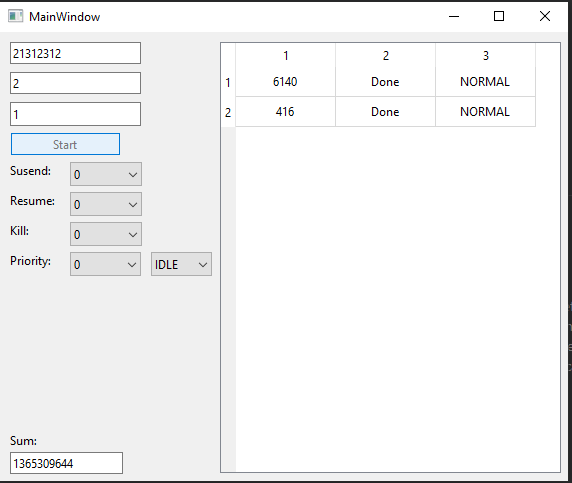
\includegraphics[scale=0.6]{v}
		\caption{Виконання програми}
	\end{figure}

	\begin{figure}[H]
		\centering
		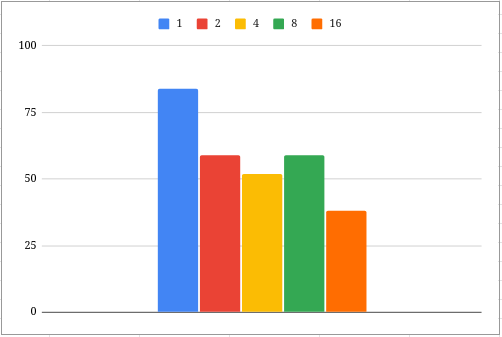
\includegraphics[scale=0.7]{1}
		\caption{Залежність часу виконання від кількості потоків}
	\end{figure}
	
	\section*{Висновок}
	Під час виконання лабораторної роботи я ознайомився з багатопоточністю в ОС Windows. Навчивсь
	реалізовувати розпаралелення алгоритмів за допомогою багатопоточності в ОС
	Windows з використанням функцій WinAPI. Навчивсь використовувати різні
	механізми синхронізації потоків
	
	 
\end{normalsize}
\end{document}
